En este capítulo se presentan diversos conceptos utilizados en este trabajo de tesis, así como definiciones relativas al problema 
y algunos algoritmos específicos relevantes para el presente trabajo.

\section{Optimización}
La optimización es un área que tiene como propósito encontrar \textit{la mejor} entre diferentes opciones elegibles. 
%
En nuestra vida diaria a menudo nos encontramos en este tipo de situaciones, por ejemplo al elegir entre diferentes rutas para 
llegar a algún lugar, o al elegir entre diferentes productos con diversas características.

En lenguaje matemático un problema de optimización consiste en minimizar o maximizar una función que le asigna un valor a cada una 
de las opciones que tenemos disponibles. 
%
Para la definición formal se adopta la siguiente notación:
\begin{itemize}
    \item $X$ El conjunto de opciones o soluciones disponibles.
    \item $f:X\rightarrow \mathbb{R}$ La función objetivo a minimizar o maximizar.
\end{itemize}

El problema consiste en hallar:
\begin{gather}
\min_{x\in X} f(x)
\end{gather}

Es importante mencionar que cualquier problema en el que se requiera encontrar el argumento que hace tomar el valor máximo a $f$ 
puede transformarse en un problema equivalente de minimización con el reemplazo $f(x) \leftarrow -f(x)$, por lo que puede considerarse 
solo el caso de minimización sin pérdida de generalidad.

En función de las características del problema y método de optimización, estos se pueden clasificar de diferentes formas. 
%
A continuación se presentan algunas de las agrupaciones más importantes.

\subsection*{Optimización con restricciones}
A la definición de un problema de optimización también pueden agregarse un conjunto de restricciones, definidas habitualmente como
un conjunto de funciones que toman una solución como entrada una solución e indican si esta cumple o no con ellas, e incluso el grado
de incumplimiento.
%
Se dice que una solución es factible si cumple con todas las restricciones e infactible en caso contrario.
%
Estas restricciones se agregan ya sea porque el problema así lo requiere o bien para asegurarse que la solución tenga sentido, por ejemplo 
si $f$ tiene como argumento un número real que representa una longitud debe requerirse que esta longitud sea un número positivo.
%
En estos casos, el problema se convierte en encontrar una solución factible que optimice la función objetivo.

\subsection*{Optimización global y local}

Hallar el mínimo de la función sobre todo el conjunto $X$ recibe el nombre de optimización global, esto puede llegar a ser muy costoso computacionalmente,
por lo que es común optar por obtener simplemente un mínimo local, es decir, una solución que sea la mejor de un subconjunto de $X$. 
%
A menudo este subconjunto se define utilizando alguna medida de distancia entre soluciones y considerando a todas las soluciones que estén en algún rango 
de distancia a otra de referencia o bien añadiendo un operador que permita crear soluciones nuevas a partir de una solución ya conocida.

\subsection*{Optimización continua y discreta}
En la definición de problema de optimización dado anteriormente no se requiere que el conjunto de soluciones tenga alguna propiedad o alguna estructura 
adicional. 
%
Por ejemplo el conjunto de soluciones puede ser un conjunto numerable ( e.g. los enteros ) o no numerable ( e.g. los números reales ). 
%
Estos dos casos dividen a la optimización en dos ramas: optimización continua y optimización discreta. 
%
En general los problemas de optimización continua suelen ser más fáciles de abordar~\cite{nocedal2006numerical} en el sentido de que se puede utilizar
el concepto de gradiente para obtener información del valor de la función objetivo de puntos cercanos a cierto punto conocido mientras que en los problemas 
discretos esto rara vez puede hacerse.
%
Sin embargo, el uso de gradientes también tiene muchas limitaciones y dificultades, por lo que ambos tipos de optimización son muy complejos y siguen
siendo tema de investigación.

\subsection*{Optimización combinatoria}
Dentro de los problemas de optimización discreta se distinguen los problemas de optimización combinatoria, en los cuales el conjunto de búsqueda es finito.
%
Los problemas de optimización combinatoria, como el tratado en esta tesis, se pueden modelar con los siguientes elementos~\cite{Blum2003}:

\begin{itemize}
    \item Un conjunto de variables $Z=\{z_1,z_2,...,z_n\}$
    \item Dominio finito para cada variable $D_1,D_2,...,D_n$
    \item Restricciones entre variables
\end{itemize}

Estos tipo de problemas aparecen en múltiples escenarios, por ejemplo cuando se requiere hallar una permutación de objetos que optimice cierta función objetivo.

\subsection*{Métodos de optimización estocástica}

En relación a los métodos de optimización, esta tesis está enfocada en los métodos estocásticos.
%
En contraste con los métodos de optimización deterministas, los métodos estocásticos pueden obtener soluciones diferentes en cada ejecución aunque tenga las mismas 
condiciones iniciales ya que internamente toman decisiones de forma probabilista.
%
En muchas ocasiones es ventajoso tener esta aleatoriedad porque nos permite explorar el espacio de búsqueda con menos sesgos, lo que es especialmente útil cuando el 
espacio de búsqueda es poco <<predecible>> en el sentido en que no podemos a priori establecer reglas que nos permitan generar soluciones que estén en regiones de alta
calidad. 
%
Uno de los método estocásticos más conocidos es recocido simulado, el cual se inspira en un fenómeno metalúrgico y que encuentra soluciones muy buenas a una gran 
variedad de problemas de optimización.
%
Posteriormente, se describen otros métodos estocásticos, incluyendo a la búsqueda local iterada, siendo este último el método que se ha utilizado en esta tesis para
validar las propuestas realizadas.


\section{Teoría de la complejidad}
De manera empírica sabemos que existen problemas <<difíciles>> y problemas <<fáciles>>, por ejemplo, es mucho más difícil armar un 
rompecabezas que comprobar que está bien armado. 
%
El área de teoría de la complejidad busca responder, entre otras, a la pregunta: \textit{¿Qué hace a algunos problemas fáciles y a 
otros difíciles?}~\cite{sipser1996introduction}. 

Uno de los logros de la teoría de la complejidad ha sido establecer un sistema de clasificación de acuerdo con la dificultad de los problemas. 
%
Este sistema consiste en muchas clases a las cuales puede ser asignado un problema en relación a los recursos computacionales necesarios para resolverlo, 
siendo las clases más estudiadas las que se definen por cantidad de operaciones (tiempo) y por memoria (espacio). 
%
A continuación se describen algunas de estas clases, así como algunas notaciones relacionadas. 

\subsection*{Notación gran $O$}
La cantidad de operaciones necesarias para resolver algún problema con un algoritmo específico puede expresarse como una función del tamaño del mismo, 
es decir de la forma $f(n)$ donde $n$ es el tamaño del problema. 
%
La función $f$ puede ser de infinidad de formas diferentes, pero para fines prácticos es de especial relevancia su comportamiento asintótico, es decir, 
cuando $n$ tiende a infinito. 
%
De esta manera se puede tener un conjunto de clases de equivalencia en las que se engloban algoritmos que tienen similar costo computacional.
%
La notación gran $O$ es usada ampliamente para describir el comportamiento asintótico de los algoritmos.

Para dos funciones $f,g:\mathbb{R}\rightarrow\mathbb{R}$ se dice que 
$f(n)= O(g(n))$\footnote{El signo de igual aquí no tiene el sentido usual sino que más bien representa una relación entre conjuntos en la que $=$ 
quiere decir $\subseteq$~\cite{graham1989concrete}} si existen constantes $c,n_0\in\mathbb{R}^+$ tal que $0\leq f(n)\leq cg(n)$ para todo 
$n\geq n_0$~\cite{cormen2009introduction}.
%
De manera intuitiva $f(n)=O(g(n))$ quiere decir que $cg(n)$ es una cota superior a $f(n)$ como puede verse en la figura \ref{fig:bigo}.

\begin{figure}[H]
    \centering
    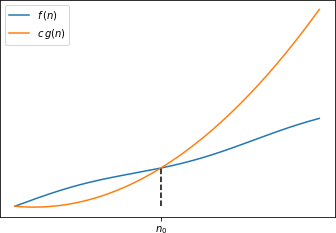
\includegraphics[scale=.8]{Imagenes/bigo.png}
    \caption{Representación de $f(n)= O(g(n))$}
    \label{fig:bigo}
\end{figure}

Se dice que un algoritmo es $O(g(n))$ si el número de operaciones que requiere para resolver un problema de tamaño $n$ es $O(g(n))$.
%
Por ejemplo, el algoritmo para sumar dos números de $n$ dígitos toma $O(n)$ operaciones (al considerar que nuestra operación básica es sumar dígitos).

\subsection*{Clases \textbf{P}, \textbf{NP} }
Un algoritmo para resolver algún problema puede tener como resultado cualquier cosa; por ejemplo un número si el problema es una suma, un polígono si buscamos una envolvente convexa, una función si resolvemos una ecuación diferencial o hasta una palabra como \texttt{sí} o \texttt{no} si buscamos saber si un número es primo.
%
Este último tipo de problema es un ejemplo de una clase importante llamada problemas de decisión. Estos problemas son de interés teórico en la teoría de la complejidad por tener una salida muy simple y porque una gran cantidad de otro tipo de problemas pueden formularse como problemas de decisión. 
%
Las clases de complejidad más analizadas están definidas para estos problemas de decisión.

%TODO: hablar de problemas de decisión
Dos de las clases más analizadas son las siguientes:

\begin{itemize} 
    \item \textbf{P}. Engloba a los problemas para los que existe un algoritmo que los resuelve y que toma a lo más $Kn^c$ operaciones con $K,c$ finitas. 
		%
		El nombre de esta clase hace referencia a que pueden resolverse en tiempo polinomial es decir que toman $O(n^c)$ operaciones para alguna $c$ positiva y finita. 

    \item \textbf{NP}. Engloba a los problemas para los que se puede verificar que se encontró una solución en tiempo polinomial. \footnote{Una definición alternativa pero equivalente se basa en el concepto de máquinas de Turing no deterministas.}
\end{itemize}

Una subclase importante de la clase \textbf{NP} es la llamada \textbf{NP-completo} que incluye a los problemas para los cuales hallar un algoritmo de solución 
en tiempo polinomial implica hallar uno para todos los problemas en \textbf{NP}. 
%
De modo intuitivo es el conjunto de los problemas más difíciles en la clase.

Claramente \textbf{P} $\subseteq$ \textbf{NP}\footnote{Si ya tenemos un algoritmo que resuelve un problema en tiempo polinomial, para verificar si una solución es correcta 
solo hay que resolver el problema} pero determinar si también se cumple esta relación en sentido contrario, es decir, determinar si \textbf{P} = \textbf{NP}, es un problema 
sumamente difícil con implicaciones importantes que no ha sido resuelto.

La distinción en algoritmos que toman tiempo polinomial podría parecer arbitraria.
%
Sin embargo, es importante porque los polinomios ejemplifican funciones de crecimiento lento y cumplen con varias propiedades teóricas que simplifican la clasificación 
de los problemas~\cite{wigderson2006p}.

%TODO: pasan a NP-hard, distinguir el JSP como NP-Completo, es decir, como problema de decisión, y el problema de optimización asociado, que es NP-hard.
%Creo que lo mejor es crear una subseción {Clase NP-hard}


\subsubsection*{Clase NP-hard}
Las clases de complejidad antes mencionadas se definieron para problemas de decisión pero son útiles para clasificar otros tipos de problemas. En particular la clase \textbf{NP-hard} sirve para clasificar problemas de optimización como el JSP . \\
Se dice que un problema de optimización pertenece a \textbf{NP-hard} si todos los problemas en \textbf{NP} pueden reducirse a él en tiempo polinomial. Para los problemas de optimización que pertenecen a esta clase no existe un algoritmo que encuentre la solución óptima en tiempo polinomial a menos que \textbf{P} = \textbf{NP}.  Es importante mencionar que el problema en cuestión no tiene por qué pertenecer a \textbf{NP}.

Muchos problemas de optimización de gran interés pertenecen a la clase \textbf{NP-hard}, entre ellos el JSP. Cabe mencionar que al JSP se le puede asociar un problema de decisión que consiste en determinar si una solución dada es óptima o no siendo este problema \textbf{NP-completo}. 
%
Ante la dificultad para resolver estos problemas de manera eficiente surgieron técnicas conocidas como metaheurísticas que buscan facilitar encontrar soluciones aceptables aunque no óptimas.





\section{Metaheurísticas}
Es muy común que en nuestra cotidianidad nos enfrentemos a problemas tan difíciles o para los que tengamos tan poco tiempo de decisión que no podamos hacer 
un análisis riguroso;
en estos casos es muy común que utilicemos algún método (posiblemente basado en la experiencia) que nos permita hallar una solución aceptable, por ejemplo, 
es común que reemplacemos el problema por uno más simple que sí podemos responder y cuya respuesta está relacionada con nuestro problema original.
%
Así, no podemos predecir con certeza si lloverá durante el día, pero sí podemos responder si el cielo está plagado de nubes oscuras.

En el contexto de la optimización, una metaheurística es una metodología de alto nivel que combina diferentes heurísticas y puede aplicarse para resolver 
de manera aproximada una gran cantidad de problemas. 
%
En la práctica existen numerosas metaheurísticas que pueden ser muy diferentes entre sí por lo que no hay un sistema de clasificación universalmente aceptado 
aunque se han propuesto diferentes criterios de clasificación~\cite{sorensen2013,Stegherr2020} con base en diferentes características:

\begin{itemize}
    \item \textbf{Poblacionales vs de trayectoria}. En las metaheurísticas poblacionales se mantiene un conjunto de soluciones candidatas que se utilizan para generar nuevas soluciones a menudo utilizando nociones de la teoría de la evolución o bien de comportamientos colectivos que se dan en la naturaleza como el comportamiento de una colonia de abejas. Por otro lado las metaheurísticas de trayectoria mantienen una única solución que se va reemplazando conforme el algoritmo avanza de modo que la solución sigue una trayectoria en el espacio de búsqueda.
    \item \textbf{Constructivas vs de mejora}. En las metaheurísticas constructivas se mantienen soluciones parciales a las que se añaden elementos hasta que se consigue una solución completa. En general suelen usar adaptaciones de algoritmos voraces para añadir estos elementos. Por otra parte en las metaheurísticas de mejora se mantienen soluciones completas que van mejorando a medida que avanza el tiempo ya sea haciendo cambios en ellas o bien reemplazándolas por nuevas soluciones mejores.
    \item \textbf{Con uso de memoria vs sin uso de memoria}. El uso de memoria consiste en almacenar información que nos ayude a explorar el espacio de búsqueda, por ejemplo una lista de soluciones previamente visitadas o una serie de características que queramos evitar o bien que sean deseables. De este modo la memoria permite tener algo parecido a un aprendizaje o a un reconocimiento de patrones en el paisaje de búsqueda que puede servir de guía.
\end{itemize} 

Si bien las metaheurísticas son muy diversas, existen elementos comunes que tienen un papel determinante en el buen funcionamiento de las mismas. 
%
En específico para las metaheurísticas de trayectoria, aunque también aplican para las demás, existen tres conceptos que determinan el llamado paisaje de búsqueda: 
la representación de las soluciones, la forma en que las soluciones están conectadas y cómo podemos compararlas entre sí. 
%
En la siguiente sección se introduce el concepto de paisaje de búsqueda y sus componentes, el cual es el principal tema de estudio de esta tesis.

\section{Paisaje de búsqueda}
El concepto de paisaje de búsqueda surgió en la biología para explicar los mecanismos de evolución de poblaciones de seres vivos~\cite{wright1932roles}. 
%
La idea básica es que los genes de algún organismo en particular le confieren ventajas o desventajas en su hábitat, i.e. puede estar más o menos adaptado. 
%
De esta manera puede pensarse en clasificar a todos los individuos de acuerdo a su grada de adaptación. 

Conforme se introducen nuevas variaciones en el código genético ya sea por la reproducción o mutación, se pueden añadir a los nuevos individuos a la clasificación. 
%
Si se continua de esta forma se obtendrá una especie de mapa en el cual podríamos asignar a cada código genético un punto en el mapa y un valor de adaptabilidad.
%
En algunas extensiones de este concepto también se agrega información sobre la procedencia de cada genoma.

El proceso previamente descrito tiene como resultado una estructura que puede representarse mediante un grafo. 
%
En el ámbito de las metaheurísticas el concepto de paisaje de búsqueda se inspira fuertemente en la descripción biológica anterior. 
%
Los conceptos de genoma, adaptabilidad y reproducción y mutación tienen como análogos la representación, la función de fitness o aptitud y la estructura de vecindad.   

\subsection{Representación}

En ocasiones, el problema de optimización en el que estemos interesados puede surgir directamente de un ámbito de las matemáticas;
%
sin embargo, si estamos interesados en un problema de nuestro entorno físico es necesario idear una forma de traducirlo a un lenguaje matemático, 
incluyendo la soluciones al mismo. 
%
Por ello, debemos encontrar una forma de representar de manera útil las soluciones posibles.
%
A continuación se considera un ejemplo sencillo donde las soluciones que buscamos son elementos de $\mathbb{R}^2$.
\subsubsection*{Ejemplo}
Supongamos que queremos colocar una lámpara en una habitación de manera que obtengamos la mejor iluminación. En este caso podemos elegir algún punto en la habitación como el origen y representar las soluciones a nuestro problema como puntos en un subconjunto de $\mathbb{R}^2$. Podemos representar estos puntos de varias maneras por ejemplo con sus coordenadas cartesianas o bien con sus coordenadas polares como en la figura \ref{fig:cartpol}.

\begin{figure}[H]
    \centering
    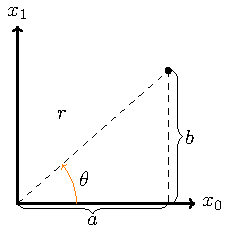
\includegraphics[scale=1.5]{Imagenes/repr_example.pdf}
    \caption{Representación en coordenadas cartesianas $(a,b)$ y polares $(r,\theta)$ para un punto  en $\mathbb{R}^2$}
    \label{fig:cartpol}
\end{figure}

Aunque son equivalentes, estas dos representaciones tienen propiedades diferentes. Por ejemplo, la representación en coordenadas polares no necesariamente es única porque $(r,\theta)$ y  $(r,\theta+2\pi)$ representan el mismo punto. Cada una de estas representaciones puede presentar ventajas o desventajas de acuerdo con factores como la forma de la habitación, tal vez sea ventajoso usar la representación cartesiana si la habitación es cuadrada o usar la representación polar si la habitación es redonda.\\

Con el ejemplo anterior también podemos ver que si queremos establecer algunos operadores que, por ejemplo, perturben la solución tendremos que definirlos de maneras 
distintas en función de la representación que estemos considerando para asegurarnos que la perturbación tiene el efecto que deseamos.
%
También es importante notar que es posible que el número de soluciones factibles e infactibles cambian en función de la representación, por lo que dependiendo de
la misma, se puede facilitar o dificultar la búsqueda.

Formalmente una representación está formada por con conjunto de objetos (representaciones de soluciones) y un mapa que asocia elementos entre el conjunto de representaciones
y el conjunto de las soluciones. 
%
Este mapeo no tiene por que ser suryectivo, es decir, que puede ser que solo asigne una representación a parte del conjunto de soluciones. 
%
También puede ser el caso como se mencionó anteriormente que haya representaciones que no correspondan a soluciones. 
%
En función del tipo de mapeo entre representaciones y soluciones se pueden distinguir las siguientes~\cite{Cheng1996}: 
\begin{itemize}
    \item $1$ a $1$ A cada solución le corresponde una única representación.
    \item $1$ a $n$ La misma representación puede asociarse a varias soluciones.
    \item $n$ a $1$ Una solución puede tener diferentes representaciones.
\end{itemize}
Una representación pictórica de los tipo de mapeo se encuentra en la figura \ref{fig:reptypes}.

Nótese que en una representación se pueden combinar las propiedades anteriores, así una solución podría estar representada por una única representación
y otra por muchas.
%
Estas características también son importantes y afectan enormemente al rendimiento de la búsqueda.

\begin{figure}[H]
    \centering
    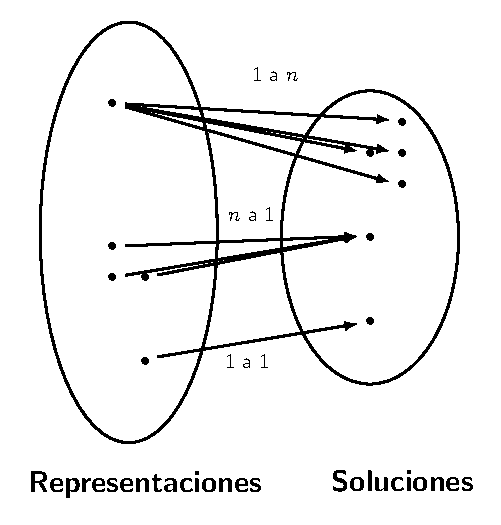
\includegraphics[scale=1]{Imagenes/representacion.pdf}
    \caption{Tipos de representaciones}
    \label{fig:reptypes}
\end{figure}

En general, el mapeo $1$ a $1$ es el más utilizado, sin embargo, todos estos tipos de mapeos han sido útiles.
%
En particular, si conseguimos un mapeo en el que las soluciones de más calidad, estén sobrerrepresentadas, se pueden conseguir búsqueda más efectivas.

\subsection{Vecindad}
La definición de vecindad es crucial para las metaheurísticas de trayectoria y las basadas en una sola solución.
%
Formalmente, una vecindad es un mapeo $N:X\rightarrow 2^X$ que le asigna a cada solución $x\in X$ un subconjunto de soluciones en $X$. 
%
Intuitivamente podemos pensar que es una forma de definir a las soluciones que <<rodean>> a otra. 
%
Se dice que la solución $y$ es un vecino de $x$ si $y\in N(x)$.

A partir de la definición de vecindad podemos también definir un operador de movimiento $M:X\rightarrow X$ cuyo efecto al aplicarlo a una solución sea 
transformarla en una que pertenezca a su vecindad, i.e. este operador selecciona a un vecino de la solución inicial.  
\[M(x)=y\in N(x)\quad x\neq y\]

En general se busca que una vecindad cumpla con ciertas características, entre las más importantes es que las soluciones formen una componente conexa, 
que no tenga un tamaño excesivamente grande y que contenga las vecinos de una solución tenga una calidad no muy distinta a la de la solución inicial;
esta última característica le confiere <<suavidad>> y puede ser de ayuda para tener búsqueda más efectivas, ya que en caso contrario, evaluar una
solución prácticamente no ofrece información sobre la calidad de la región en la que se está buscando.

\subsection{Funci\'on de aptitud o fitness}
En el momento en el que se define el problema de optimización, se define cuál es la función objetivo; 
no obstante, puede resultar útil construir otra función a la cual se le conoce como función de aptitud o fitness que toma en cuenta otras características 
de las soluciones para que el paisaje de búsqueda tenga una estructura más favorable para los métodos de solución que se pretendan usar. 
%
Por ejemplo puede suceder que aunque dos soluciones tengan asociado el mismo valor de la función objetivo una de ellas posea características que la hacen 
un mejor punto de partida para alguna metaheurística.
%
Por ello, el diseño de funciones de aptitud o fitness apropiadas es muy importante para el buen desempeño de los algoritmos.

La función de aptitud debe asociar a cada solución un elemento de un conjunto en que se tiene definida una noción de ordenamiento. 
%
En esencia esta función define un operador de comparación entre soluciones de modo que define qué soluciones se consideran mejor que otras.
%
Una vez que tenemos el conjunto de soluciones representables y operadores de cambio para generar nuevas soluciones a partir de otras, se define 
el espacio de búsqueda como un grafo dirigido $G$ en el que los nodos son las soluciones al problema y una solución $x$ está conectada a otra $y$ 
si podemos generar a $y$ aplicando los operadores de cambio a $x$.

Además, podemos asociar a cada solución en el espacio un valor de aptitud o fitness que mide la calidad de dicha solución. 
%
La adición de esta función de aptitud al espacio de búsqueda genera al paisaje de búsqueda. 
%
Formalmente el paisaje de búsqueda $\mathcal{L}$ es entonces una tupla conformada por el espacio de búsqueda junto con una función objetivo que 
guía la búsqueda $\mathcal{L}=(G,f)$.

En la figura \ref{fig:landscape} se muestra una representación pictórica del paisaje de búsqueda para un problema de optimización.

\begin{figure}
\begin{subfigure}{.4\textwidth}
    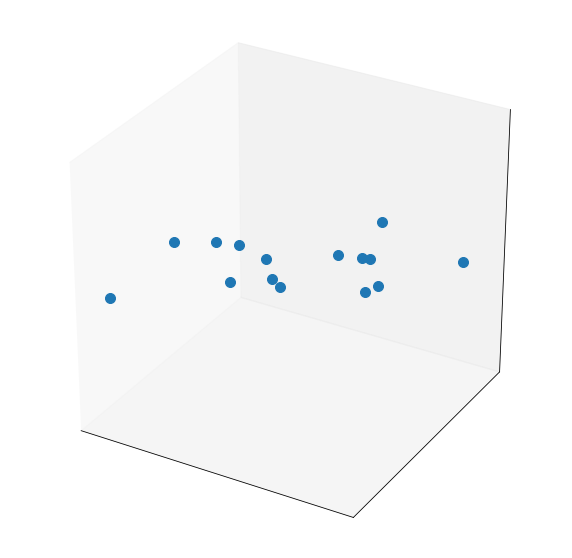
\includegraphics[scale=.5]{Imagenes/search1.png}
    \caption{Soluciones representables}
\end{subfigure}
\begin{subfigure}{.5\textwidth}
    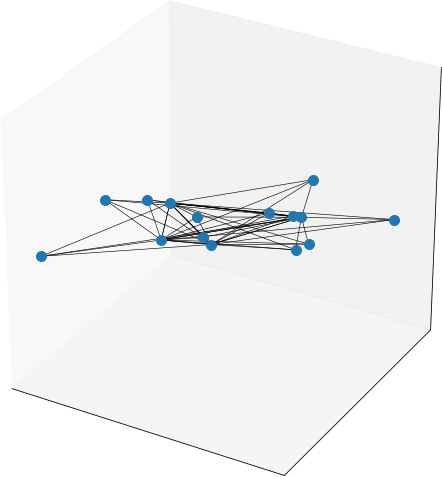
\includegraphics[scale=.5]{Imagenes/search2.png}
    \caption{Relaciones inducidas por los operadores de cambio}
\end{subfigure}
\begin{subfigure}{\textwidth}
    \centering
    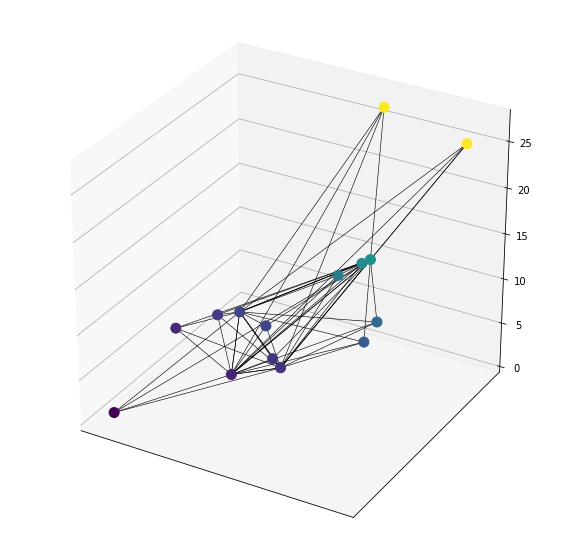
\includegraphics[scale=.5]{Imagenes/search3.png}
    \caption{Adición de la función de fitness}    
\end{subfigure}
\caption{Creación del paisaje de búsqueda}
\label{fig:landscape}
\end{figure}

\medskip
El paisaje de búsqueda es el <<terreno>> a explorar y puede cambiar si cambiamos cualquiera de sus componentes.
%
Así, podría ser que alguna representación nos centre en un subconjunto de soluciones convenientes o que se proponga alguna estructura de vecindad 
de modo que las mejores soluciones nunca están muy lejos del resto, o que la función de fitness nos ayude a atravesar cúmulos de soluciones que serían iguales si se usara
directamente la función objetivo.

La estructura del paisaje de búsqueda influye de manera determinante en el éxito o fracaso de las metaheurísticas. 
%
Dependiendo de la <<forma>> del paisaje se favorecerá el uso de ciertas metaheurísticas. 
%
La <<forma>> del paisaje hace referencia a cómo cambia el valor de fitness para soluciones conectadas entre sí y para modelarlo de forma adecuada se usan diferentes
tipos de mediciones. En la figura \ref{fig:landtypes} se muestran los diferentes tipos de paisajes de búsqueda.
%
Una medida ampliamente usada estima cómo cambia el valor de la función de fitness conforme nos acercamos a óptimos locales, mientras que otra se gran popularidad 
estima qué tanto cambia el fitness entre soluciones vecinas\cite{skauffman}. 
%
La primera de estas medidas nos da una idea de qué tan grandes son los valles que rodean a un mínimo local si es que existen y la segunda nos da una ida de la 
rugosidad del paisaje.
%
En esta tesis no nos centramos en cómo cuantificar y analizar el paisaje de búsqueda, por lo que no se entra en más detalle.
%
El objetivo se centra en proponer modificaciones a los paisajes de búsqueda más usado para el JSP, con el fin de mejorar el rendimiento de metaheurísticas sencillas.

% imagen
\begin{figure}[]
\begin{subfigure}{.45\textwidth}
    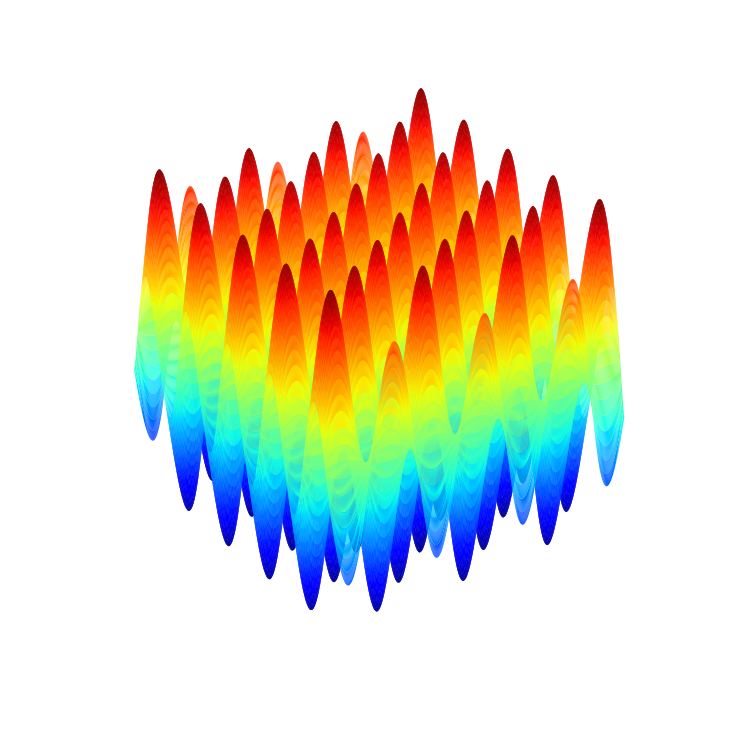
\includegraphics[scale=.4]{Imagenes/rugged.png}
    \caption{Paisaje rugoso con muchos óptimos locales}
\end{subfigure}
\begin{subfigure}{.5\textwidth}
    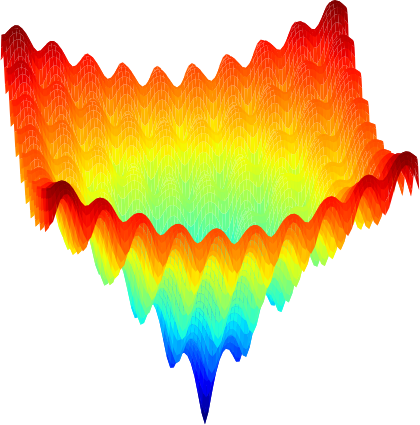
\includegraphics[scale=.4]{Imagenes/ruggedvalley.png}
    \caption{Paisaje rugoso con con un gran valle}
\end{subfigure}
\begin{subfigure}{\textwidth}
    \centering
    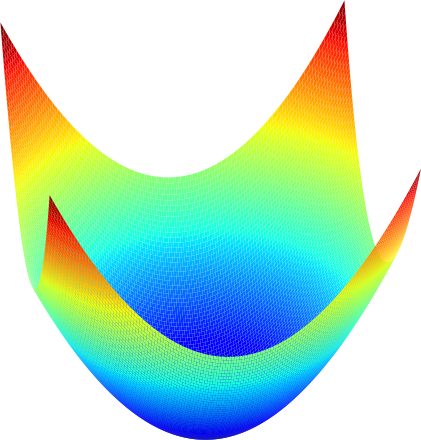
\includegraphics[scale=.4]{Imagenes/smoothvalley.png}
    \caption{Paisaje suave con un gran valle}
\end{subfigure}
\caption{Diferentes tipos de paisajes de búsqueda. Se muestran paisajes continuos con fines ilustrativos.}
    \label{fig:landtypes}
\end{figure}

\subsection*{Algunas metaheurísticas de relevancia}
Las metaheurísticas sirven como una estrategia para explorar el paisaje de búsqueda. 
%
Una de las más sencillas e intuitivas es conocida como descenso/escalada estocástica y simplemente consiste en reemplazar la solución actual por algún vecino mejor 
escogido al azar .%
Esta es una metaheurística de trayectoria y traza un camino entre las soluciones inicial y final.

%
\begin{algorithm}[H]
 \KwData{Problema de Optimización}
    \KwResult{Óptimo local $x$}
 Generar solución inicial $x$\;
 Generar lista de vecinos $L$ de $x$\;
 \While{$L$ no vacía}{
    Generar lista de vecinos $L$ de $x$\;
    Escoger al azar un vecino $y\in L$\;
  \eIf{$y<x$}{
      $x \leftarrow y$\;
      Generar lista de vecinos $L$ de $x$\;
   }{
       Quitar a $y$ de $L$\;
  }
 }
    \Return{x}
    \label{alg:LS}
    \caption{Algoritmo de descenso/escalada estocástica}
\end{algorithm}

\begin{figure}[H]
\centering
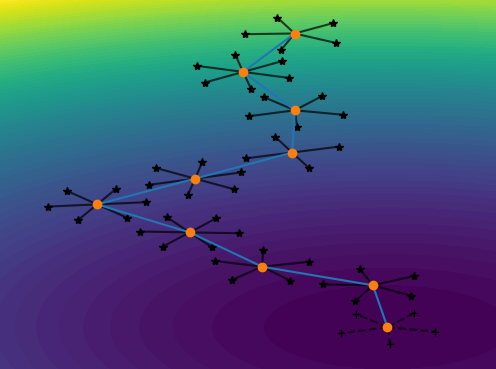
\includegraphics[scale=.8]{Imagenes/mettray.png}
    \caption{Ilustración de un descenso estocástico. Las aristas rayadas representan la vecindad del óptimo local.}
\end{figure}


Otra metaheurística de trayectoria importante que se ha considerado en la mayor parte de métodos que han alcanzado las mejores soluciones conocidas para el JSP es
la llamada búsqueda tabú \ref{alg:TS}. 
%
Esta metaheurística se basa en la búsqueda local pero puede aceptar vecinos que no mejoran la función de fitness con la intención de evitar atascarse en un óptimo 
local de mala calidad. 
%
La búsqueda tabú almacena soluciones previamente vistas o características de las mismas para evitar visitarlas de nuevo. 
%
De entre las soluciones vecinas no prohibidas por la lista tabú, se mueve a la mejor.
%
Es necesario definir el tamaño de la lista, el tipo de información que contendrá y el criterio de paro.

\begin{algorithm}[H]
 \KwData{Problema de Optimización}
 \KwResult{Mejor solución encontrada $x^*$}
 Generar solución inicial $x$\;
    Inicializar mejor solución como $x^*\leftarrow x$
 Inicializar la lista tabú $TL$ con información de $x$ \; 
 \While{no criterio de paro}{
    Generar lista de vecinos $L$\;
    Escoger un vecino $y\in L$ que no esté prohibido por $TL$ \;
      $x \leftarrow y$\;
      Actualizar $TL$\;
      \If{$x<x^*$}{
      $x^* \leftarrow x$\;
      }
 }
    \Return{$x^*$}
    \label{alg:TS}
    \caption{Algoritmo básico de búsqueda tabú}
\end{algorithm}

\smallskip
Por último se presenta una metaheurística de trayectoria muy sencilla que intenta subsanar el problema de atascarse en óptimos locales de mala calidad de la búsqueda local,
la búsqueda local iterada \ref{alg:ILS}.
%
La idea de esta metaheurística es obtener un mínimo local a partir de una solución inicial mediante búsqueda local, y aplicarle una perturbación seguida de búsqueda local para
evitar el óptimo local.
%
Este proceso se repite hasta que se cumpla algún criterio de paro. 
%
Esta estrategia es conceptualmente muy simple aunque se debe definir la perturbación que se hace a la solución y por lo general no es tan sencillo plantear una perturbación adecuada. También debe definirse un criterio de aceptación para las soluciones, lo más común es que se pida que la nueva solución tenga un valor de fitness mejor que la anterior, como es el caso en este trabajo.\\

\begin{algorithm}[H]
 \KwData{Problema de Optimización}
 \KwResult{Última solución aceptada $x^*$}
 Generar solución inicial $x$\;
 Inicializar mejor solución como $x^*\leftarrow x$
 \While{no criterio de paro}{
     Obtener una solución $y$ a partir de $x$ mediante búsqueda local \ref{alg:LS}\;
     \eIf{$y$ es aceptada}{
     $x \leftarrow y$\;
     $x^* \leftarrow y$\;
    }{
     $x \leftarrow x^*$\;
     Perturbar $x$\;
    }
 }
    \Return{$x^*$}
    \label{alg:ILS}
    \caption{Algoritmo búsqueda local iterada}
\end{algorithm}
